% Generated by code/scripts/report_figures.py at 2026-11-04T14:50:10Z; do not edit.
% Inputs: artifacts/cluster/runs/gpu_timing-20261104T111747Z-1519638
\begin{figure}[t]
\centering
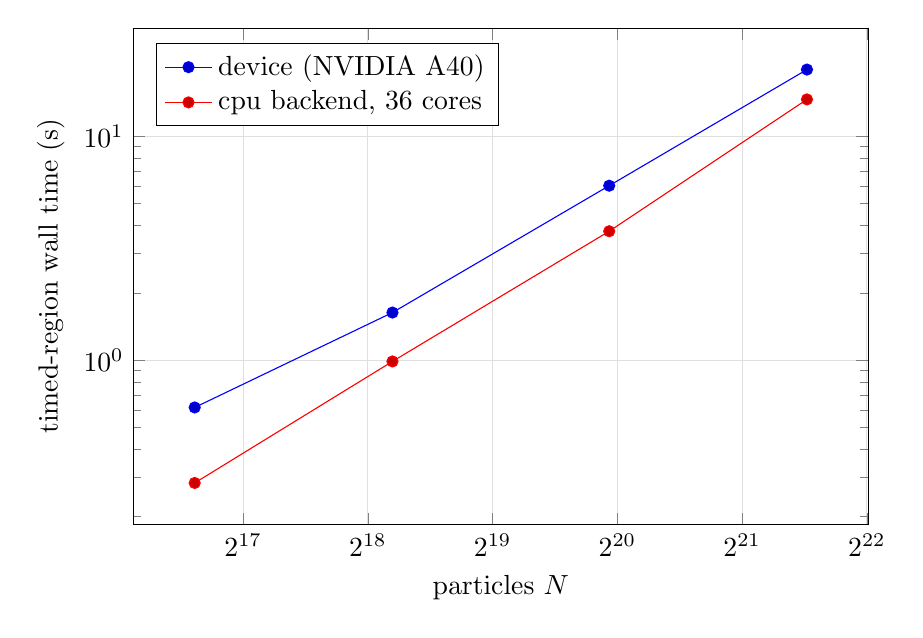
\begin{tikzpicture}
\begin{axis}[width=0.9\columnwidth, height=0.65\columnwidth, xlabel={particles $N$}, ylabel={timed-region wall time (s)}, xmode=log, log basis x=2, ymode=log, legend pos=north west, legend cell align=left, grid=major, grid style={gray!25}]
\addplot+[mark=*] coordinates {(100000,0.6153) (300000,1.633) (1e+06,6.019) (3e+06,19.87)};
\addlegendentry{device (NVIDIA A40)}
\addplot+[mark=*] coordinates {(100000,0.2831) (300000,0.9878) (1e+06,3.768) (3e+06,14.62)};
\addlegendentry{cpu backend, 36 cores}
\end{axis}
\end{tikzpicture}
\caption{Same program and workloads on the device and CPU backends, median of repetitions. 5 timed steps, $\theta=0.5$, leaf size 8, Intel(R) Xeon(R) Platinum 8452Y. Only the force traversal differs: on the device, or on 36 bound CPU threads (schedule dynamic, chunk 64). Both backends build and flatten the tree and integrate on one host thread, and those times are included; setup and warmup are not.}
\label{fig:gpu-runtime}
\end{figure}
